% SC2203 --- Chapter 3: Properties of Regular Languages (0->100 ground-up)
\chapter{Properties of Regular Languages}
\label{ch:regular-properties}

\begin{quote}
\emph{``How do we prove a language is \emph{not} regular?''} --- DFAs have finite memory; a language needing unbounded counting cannot be regular. Pumping and Myhill--Nerode make this precise, and minimisation squeezes every DFA to its canonical core.
\end{quote}

\noindent\fbox{\parbox{\dimexpr\linewidth-2\fboxsep-2\fboxrule}{%
\textbf{From zero: we build here, no prior distinguishability assumed.} We start from the pigeonhole principle, then state pumping, then the stronger Myhill--Nerode characterisation, then DFA minimisation as partition refinement. Everything proved from definitions in Ch.~2.}}
\vspace{0.4em}

\section*{Learning Outcomes}
After this chapter you will be able to:
\begin{enumerate}[label=(L\arabic*)]
    \item state and apply the pumping lemma for regular languages;
    \item choose a witness $w$ and pump to prove non-regularity (e.g.\ $0^n1^n$, palindromes);
    \item state Myhill--Nerode and count equivalence classes to prove (non-)regularity;
    \item explain closure properties and how they combine with pumping/Myhill--Nerode;
    \item minimise a DFA via table-filling / partition refinement and argue uniqueness.
\end{enumerate}

% ============================================================
\section{Why Some Languages Need Infinite Memory}
\label{sec:why-nonregular}
A DFA with $p$ states reading a word of length $\ge p$ must repeat a state (pigeonhole). The loop between the two visits can be repeated or deleted---this is the seed of pumping.

% TikZ 1: pigeonhole loop diagram
\begin{figure}[h]
\centering
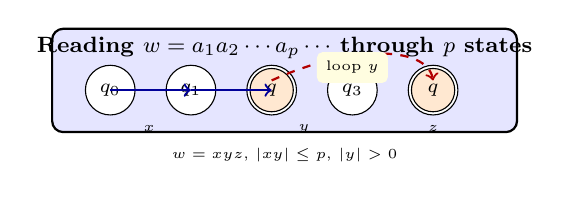
\begin{tikzpicture}[scale=0.82,every node/.style={font=\scriptsize}]
\draw[thick,fill=blue!10,rounded corners=4pt] (0,0) rectangle (7.2,1.6);
\node[font=\footnotesize\bfseries] at (3.6,1.3) {Reading $w=a_1a_2\cdots a_p\cdots$ through $p$ states};
\foreach \i in {0,1,2,3,4} {\node[draw,circle,fill=white,minimum size=0.55cm] at (0.9+1.25*\i,0.65) {$q_{\i}$};}
\node[draw,circle,fill=orange!18,minimum size=0.55cm] at (0.9+1.25*2,0.65) {$q$};
\node[draw,circle,fill=orange!18,minimum size=0.55cm] at (0.9+1.25*4,0.65) {$q$};
\draw[->,thick,blue!60!black] (0.9,0.65) -- (2.15,0.65);
\draw[->,thick,blue!60!black] (2.15,0.65) -- (3.4,0.65);
\draw[->,thick,red!70!black,dashed] (3.4,0.80) .. controls (4.6,1.35) and (5.8,1.35) .. (5.9,0.80);
\node[font=\tiny,fill=yellow!12,rounded corners=2pt] at (4.65,1.0) {loop $y$};
\node[font=\tiny] at (1.5,0.05) {$x$};
\node[font=\tiny] at (3.9,0.05) {$y$};
\node[font=\tiny] at (5.9,0.05) {$z$};
\node[font=\tiny] at (3.6,-0.35) {$w=xyz$, $|xy|\le p$, $|y|>0$};
\end{tikzpicture}
\caption{Pigeonhole forces a repeat: $w=xyz$ where $y$ loops on the repeated state; $xy^iz$ stays accepted.}
\label{fig:pigeonhole-loop}
\end{figure}

% ============================================================
\section{The Pumping Lemma for Regular Languages}
\label{sec:pumping}
\begin{theorem}[Pumping lemma, regular]
If $L$ regular then $\exists p\ge1$ (pumping length) such that $\forall w\in L$ with $|w|\ge p$, $\exists$ split $w=xyz$ with (i) $|xy|\le p$, (ii) $|y|>0$, (iii) $\forall i\ge0:\;xy^iz\in L$.
\end{theorem}
\begin{proof}
Take DFA $M$ for $L$ with $p=|Q|$ states. Trace $w$ of length $\ge p$: the $p+1$ prefixes visit $p+1$ states, so some state repeats within first $p$ symbols. Let $x$ lead to first visit, $y$ the loop, $z$ the rest: $|xy|\le p$, $|y|>0$, and looping $y$ any $i$ times stays in the same accept/reject status. \qed
\end{proof}

\emph{Contrapositive use:} to show $L$ not regular, pick for each $p$ a long $w\in L$ and show \emph{every} admissible $x,y,z$ fails to pump.

\begin{example}[Classic $0^n1^n$ is not regular]
$L=\{0^n1^n\mid n\ge0\}$. Assume regular with $p$. Choose $w=0^p1^p\in L$, $|w|\ge p$. Any split $xyz$ with $|xy|\le p$ forces $y=0^k$, $k>0$, lying entirely in the $0$-block. Then $xy^2z=0^{p+k}1^p\notin L$ (too many $0$s), violating (iii). Contradiction. Hence $L$ not regular. Same idea shows $\{0^n1^n\mid n\ge1\}$, $\{ww\mid w\in\{0,1\}^*\}$ not regular.
\end{example}

\begin{example}[Palindromes not regular]
$L=\{w\mid w=w^R\}$ over $\{0,1\}$. Take $w=0^p10^p\in L$ (even length with centre $1$). Any $y$ in first $p$ symbols is $0^k$, pumping disrupts symmetry: $xy^2z=0^{p+k}10^p\notin L$. The crucial point is $|xy|\le p$ pins $y$ to the left block.
\end{example}

% TikZ 2: pumping adversarial game tree
\begin{figure}[h]
\centering
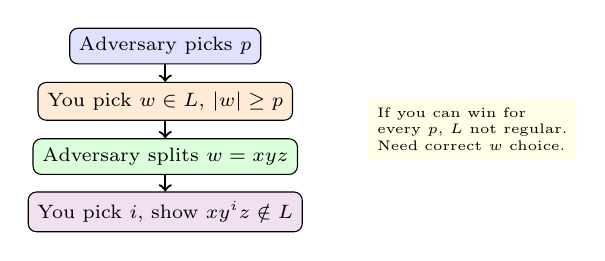
\begin{tikzpicture}[scale=0.78,every node/.style={font=\scriptsize}]
\node[draw,fill=blue!12,rounded corners=3pt] (a) at (0,2.0) {Adversary picks $p$};
\node[draw,fill=orange!16,rounded corners=3pt] (b) at (0,1.1) {You pick $w\in L$, $|w|\ge p$};
\node[draw,fill=green!14,rounded corners=3pt] (c) at (0,0.2) {Adversary splits $w=xyz$};
\node[draw,fill=violet!12,rounded corners=3pt] (d) at (0,-0.7) {You pick $i$, show $xy^iz\notin L$};
\draw[->,thick] (a)--(b); \draw[->,thick] (b)--(c); \draw[->,thick] (c)--(d);
\node[font=\tiny,align=left,fill=yellow!10,rounded corners=2pt] at (5.0,0.65) {If you can win for\\every $p$, $L$ not regular.\\Need correct $w$ choice.};
\end{tikzpicture}
\caption{The pumping game: existential/universal quantifiers as a game; winning strategy proves non-regularity.}
\label{fig:pumping-game}
\end{figure}

\begin{remark}[Common pitfalls]
Pumping lemma is necessary but not sufficient; there are non-regular languages that still pump (e.g.\ $\{a^ib^jc^k\mid i=0\text{ or }j=k\}$). Use Myhill--Nerode for a complete characterisation. Also $w$ must be chosen wisely: $0^p1^p$ works, but $0^p1^{p}$ with $i=0$ vs.\ $2$ matters---always exhibit one $i$ that breaks membership.
\end{remark}

% ============================================================
\section{Myhill--Nerode: The Exact Criterion}
\label{sec:myhill-nerode}
Define $x\sim_L y$ iff $\forall z\in\Sigma^*,\;xz\in L\Leftrightarrow yz\in L$ (indistinguishable extensions). $\sim_L$ is an equivalence; its classes partition $\Sigma^*$.

\begin{theorem}[Myhill--Nerode]
$L$ regular iff $\sim_L$ has finitely many classes. Number of classes = number of states of the minimal DFA for $L$.
\end{theorem}
\begin{proof}[Sketch]
($\Rightarrow$) DFA with $|Q|$ states puts strings reaching the same state into the same class: at most $|Q|$ classes. ($\Leftarrow$) Build DFA whose states \emph{are} the classes: $\delta([x],a)=[xa]$, $q_0=[\varepsilon]$, $F=\{[x]\mid x\in L\}$. Well-defined and minimal because any DFA must separate distinguishable strings. \qed
\end{proof}

\begin{example}[0$^n$1$^n$ has infinitely many classes]
For $x_m=0^m$ and $x_n=0^n$ with $m\neq n$, take $z=1^m$: $x_mz=0^m1^m\in L$ but $x_nz=0^n1^m\notin L$, so $x_m\not\sim_L x_n$. Hence infinitely many distinct classes $\{0^n\}$; $L$ not regular and no finite DFA exists.
\end{example}

\begin{example}[When Myhill--Nerode is easier]
$L=\{w\mid\#_0(w)=\#_1(w)\}$ (balanced, not $0^*1^*$). For $x_k=0^k$, $z=1^k$ distinguishes, giving infinite classes---one-line proof vs.\ tricky pumping. Even $L=\{a^nb^n\mid n\ge0\}\cup\{b^n a^n\}$ also needs Myhill--Nerode.
\end{example}

\begin{example}[Code: distinguishability test]
\begin{lstlisting}[language=Python]
def distinguish(L, x, y, bound=6):
    # brute-force search for separating extension z up to bound
    from itertools import product
    Sigma=['0','1']
    for l in range(bound+1):
        for z in product(Sigma, repeat=l):
            z=''.join(z)
            if (x+z in L) != (y+z in L):
                return z  # z separates x,y
    return None
# distinguish({0n1n}, '00','000') -> '11' separates
\end{lstlisting}
For regular $L$, this search terminates by Myhill--Nerode finiteness; for non-regular, it may need unbounded $z$.
\end{example}

\begin{theorem}[Regular pumping vs.\ Myhill--Nerode strength]
If $\sim_L$ has $p$ classes then $p$ is a pumping length. Conversely, a language can pump with $p$ yet have infinitely many $\sim_L$-classes (pumping is strictly weaker).
\end{theorem}
\begin{proof}[Sketch]
If $p$ classes, among $p+1$ prefixes of any $|w|\ge p$ two fall in same class; their difference loop pumps. Counterexample for converse is the Bar-Hillel language above; pumping holds vacuously for short witnesses but distinguishability still infinite. \qed
\end{proof}

% ============================================================
\section{DFA Minimisation}
\label{sec:minimisation}
Among all DFAs for $L$, one is smallest (up to isomorphism). Minimise by merging indistinguishable states.

% TikZ 3: minimisation partition refinement
\begin{figure}[h]
\centering
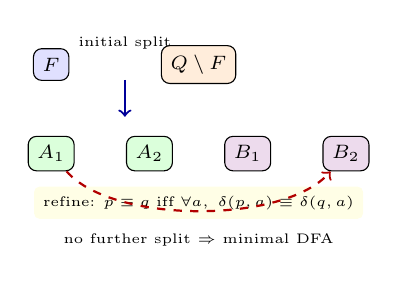
\begin{tikzpicture}[scale=0.78,every node/.style={font=\scriptsize}]
\node[draw,fill=blue!12,rounded corners=3pt] (s0) at (0,1.2) {$F$};
\node[draw,fill=orange!14,rounded corners=3pt] (s1) at (2.4,1.2) {$Q\setminus F$};
\node[font=\tiny] at (1.2,1.55) {initial split};
\draw[->,thick,blue!60!black] (1.2,0.95)--(1.2,0.35);
\node[draw,fill=green!14,rounded corners=3pt] (t0) at (0,-0.25) {$A_1$};
\node[draw,fill=green!14,rounded corners=3pt] (t1) at (1.6,-0.25) {$A_2$};
\node[draw,fill=violet!14,rounded corners=3pt] (t2) at (3.2,-0.25) {$B_1$};
\node[draw,fill=violet!14,rounded corners=3pt] (t3) at (4.8,-0.25) {$B_2$};
\node[font=\tiny,fill=yellow!10,rounded corners=2pt] at (2.4,-1.05) {refine: $p\equiv q$ iff $\forall a,\;\delta(p,a)\equiv\delta(q,a)$};
\draw[->,thick,red!70!black,dashed] (t0) .. controls (1.0,-1.4) and (3.8,-1.4) .. (t3);
\node[font=\tiny,align=center] at (2.4,-1.65) {no further split $\Rightarrow$ minimal DFA};
\end{tikzpicture}
\caption{Table-filling / partition refinement: start $\{F,Q\setminus F\}$, repeatedly split blocks whose $a$-successors land in different blocks; remaining blocks are the minimal states.}
\label{fig:minimisation}
\end{figure}

Algorithm (table-filling, $O(|Q|^2|\Sigma|)$): mark pairs $(p,q)$ with $p\in F\not\ni q$ as distinguishable; iteratively mark $(p,q)$ if $\exists a$ with $(\delta(p,a),\delta(q,a))$ already marked. Unmarked pairs are equivalent---merge them. Hopcroft's $O(|\Sigma||Q|\log|Q|)$ is the fast variant.
\begin{remark}[Why minimise?]
Minimal DFA is the Myhill--Nerode DFA; any larger DFA wastes states that are indistinguishable. Minimisation also gives a decision procedure for equivalence: minimise both DFAs and check isomorphism (up to renaming)---linear after minimisation.
Brzozowski's double-reversal trick also yields the minimal DFA and is often simpler to implement than table-filling.
In practice, keep DFAs minimal after each product/closure to prevent state explosion.
\end{remark}

\begin{example}[Minimising ``ends with $01$'' DFA]
Subset DFA from Ch.~2 had $4$ states: $\{0\},\{0,1\},\{0,2\},\{0\}$? Actually $3$ reachable non-equivalent. Table-filling finds $\{0\}$ and $\{0,2\}$ distinguishable from others but $\{0\}$ initial and final? Ends with $01$ minimal DFA has $3$ states (residuals: $\varepsilon$, $0$, $01$). No two merge, so already minimal. A DFA with an extra dead trap plus duplicate accept can be collapsed to this.
\end{example}

% ============================================================
\section{Closure and Decidability Preview}
\label{sec:closure-decidable}
Regular languages are closed under $\cup,\cap,\overline{\ },\cdot,*,R$, homomorphism and inverse homomorphism. Each closure has a constructive automaton, yielding decidability: emptiness ($F$ reachable from $q_0$?), universality ($\overline{L}=\emptyset$?), inclusion ($L_1\setminus L_2=\emptyset$?), equivalence ($L_1\oplus L_2=\emptyset$?) are all decidable via graph reachability on automata. Finiteness is also decidable via pumping length $p$: check strings up to $p$ and $p$--$2p$.

\begin{example}[Closure in action]
To decide if $L=\{0^n1^n\}$ were regular (it is not), intersect with regular $0^*1^*$ does nothing; but $L_1=\{a^mb^n\mid m\neq n\}$ is $a^*b^*\setminus\{a^nb^n\}$; if $\{a^nb^n\}$ were regular its complement in $a^*b^*$ would be too. Using closure we transport non-regularity without repeating pumping. Complement flips $F$; product gives $\cap$; De Morgan gives $\cup$.
\end{example}

\begin{theorem}[Decidability of emptiness etc.]
Given DFA $M$, $L(M)=\emptyset$ iff no accept state reachable from $q_0$ (BFS $O(|Q|+|\delta|)$). Hence universality, inclusion, equivalence are decidable: $L_1\subseteq L_2$ iff $L_1\cap\overline{L_2}=\emptyset$; $L_1=L_2$ iff both inclusions hold.
\end{theorem}

% ============================================================
\section{Chapter Notes}
Pumping lemma folklore (Bar-Hillel); Myhill--Nerode (1957--58) gives the definitive test and minimisation correctness. Brzozowski's minimisation (reverse--determinise--reverse--determinise) is an elegant alternative.
Hopcroft's $O(n\log n)$ partition refinement is optimal for minimisation and mirrors DFA learning.
Non-closure of decidability beyond regular is the theme of Ch.~7: emptiness stays decidable for CFLs but equivalence does not.
For practice, implement table-filling in Python and test on random DFAs; minimal DFAs are unique up to renaming, giving a canonical form for $L$.
Reachability plus minimisation reduces many regular-language questions to graph algorithms.

% ============================================================
\section{Exercises}
\label{sec:ch03-exercises}
\begin{enumerate}[label=E3.\arabic*, leftmargin=*, itemsep=0.8em]
\item \textbf{Pumping warm-up.} Prove $L=\{0^n1^n2^n\mid n\ge0\}$ not regular in two ways: (a) pumping, (b) Myhill--Nerode via $0^n$. Which is shorter?
\item \textbf{Closure vs.\ pumping.} Show $L=\{a^mb^n\mid m\neq n\}$ not regular using closure under complement/intersection with $a^*b^*$. Why does a direct pump with $w=a^pb^p$ need care?
\item \textbf{Myhill--Nerode counting.} For $L=\{w\mid w$ ends with $010\}$, compute $|\Sigma^*/\!\sim_L|$ and build minimal DFA; exhibit distinguishing extensions for each pair of residuals.
\item \textbf{Minimisation trace.} Minimise DFA with $Q=\{A,B,C,D,E\}$, $F=\{C\}$, $\delta$ given by table (provide). Use table-filling, list marked pairs in order, give quotient DFA and argue minimality via Myhill--Nerode.
\item \textbf{Pumping is not sufficient.} Give a non-regular $L$ that satisfies the pumping lemma (hint: $\{a^ib^jc^k\mid i=0\text{ or }j=k\}\cup a^*b^*$) and explain why Myhill--Nerode still detects non-regularity (infinitely many $b^jc^k$ classes).
\end{enumerate}
% End of Chapter 3
